%================================================================
\chapter{Models of Neural Dynamics}\label{chap:compneuro}
%================================================================

Understanding the complex mechanisms of the nervous system requires the construction and analysis of models of neural dynamics at different levels. In this chapter, we discuss the seminal Hodgkin-Huxley model \cite{HH1952} that is a biophysically detailed description of the ionic mechanisms underlying the initiation and propagation of action potentials in squid giant axons. We also consider the Brunel network model \cite{Brunel2000} for activity dynamics in local cortical networks. The content of this chapter is mainly based on \cite{Sterratt}, \cite{dayan_abbott} and \cite{neuro_dynamics}.


%================================================================
\section{The Hodgkin-Huxley Model}\label{sec:hh_model}
%================================================================ 

The Hodgkin-Huxley (HH) model was the first quantitative model of active membrane properties, and gave a biophysically detailed description of the mechanisms that give rise to action potentials (APs) in neurons. The model was used to compute the shape of action potentials in the squid giant axon. The model, and the experimental work that led up to it, earned its authors a share of the 1963 Nobel Prize in Physiology or Medicine, establishing a new framework for thinking about the electrical activity of neurons. Before we present the model itself, we first briefly discuss the basics of mathematical modeling of neurons. 


%================================================================
\subsection{Electrical Properties of Neurons}
%================================================================ 

The basis of electrical activity in neurons is the flow of ions into and out of the neuron through ion channels in the neuronal membrane. As ions are electrically charged, they exert forces on and experience forces from other ions. The force acting on an ion is proportional to the ion's charge, $q$. As we established in the previous chapter, there is typically an excess negative charge on the inside surface of the neuron and a balancing positive charge on its outer surface. The lipid bilayer forms an insulating barrier between the outside and interior of the neuron. As such, the neuronal membrane behaves as a \textit{capacitor}, described by:

\begin{equation}\label{eq:capacitor}
    q = C_m V,
\end{equation}

where $V$ is the membrane potential and the constant of proportionality $C_m$ the membrane capacitance, which indicates how much charge can be stored on a particular capacitor for a given potential difference across it. All current passing through the membrane either charges or discharges the membrane capacitance, so the rate of change of charge, $\dd{q}/\dd{t}$, on the membrane is the same as the net current, $I$, flowing through the membrane: $I=\dd{q}/\dd{t}$. By differentiating \autoref{eq:capacitor}, we can use the membrane capacitance to determine how much current is required to change the membrane potential at a given rate: 

\begin{equation}\label{eq:dVdt_fundamental}
   C_m \frac{\dd{V}}{\dd{t}} = \frac{\dd{q}}{\dd{t}} = I.
\end{equation} 

\autoref{eq:dVdt_fundamental} is fundamental in the mathematical modeling of neurons, as it relates how the membrane potential evolves over time with the net flow of current through ion channels. It should be noted that in the context of modeling the entire neuron, $C_m$ is technically the membrane capacitance per unit area. The current $I_\mathrm{X}$ per unit area through an ion channel of type $X$ is modelled by the quasi-ohmic relation: 

\begin{equation}
    I_\mathrm{X} = g_\mathrm{X} \qty(V - \mathrm{E_X}),
\end{equation}

where $g_\mathrm{X}$ is the \textit{conductance} of the specific ion channel per unit area and $E_\mathrm{X}$ the reversal potential of ion $\mathrm{X}$. $\qty(V - \mathrm{E_X})$ is called the \textit{driving force}, and when the membrane potential is at the reversal potential for ion $\mathrm{X}$, the driving force is zero. The conductance is a measure of the ease with which an electric current passes, and is the reciprocal of the resistance. The total current per unit area across the neuronal membrane, $I$, is the sum of the contributions from the different types of ion channels:

\begin{equation}
    I = \sum_\mathrm{X} g_\mathrm{X} \qty(V - \mathrm{E_X}).
\end{equation}


%================================================================ 
\subsection{Biophysical Model of Ionic Mechanisms}
%================================================================ 

From a biophysical point of view, APs are the result of ionic currents that pass through the neuronal membrane. In an extensive series of electrophysiology experiments on the squid giant axon, Hodgkin and Huxley succeeded to measure these currents and to describe their dynamics in terms of differential equations. Hodgkin and Huxley treated the squid giant axon as an equivalent electrical circuit, see \autoref{fig:hh_circuit}, with the current across the membrane being carried by either a capacitor current, $I_\mathrm{C}$, current of potassium ions, $I_\mathrm{K}$, current of sodium ions, $I_\mathrm{Na}$ or a catch-all leakage current, $I_\mathrm{L}$. 
\begin{figure}[!htb]
    \centering
    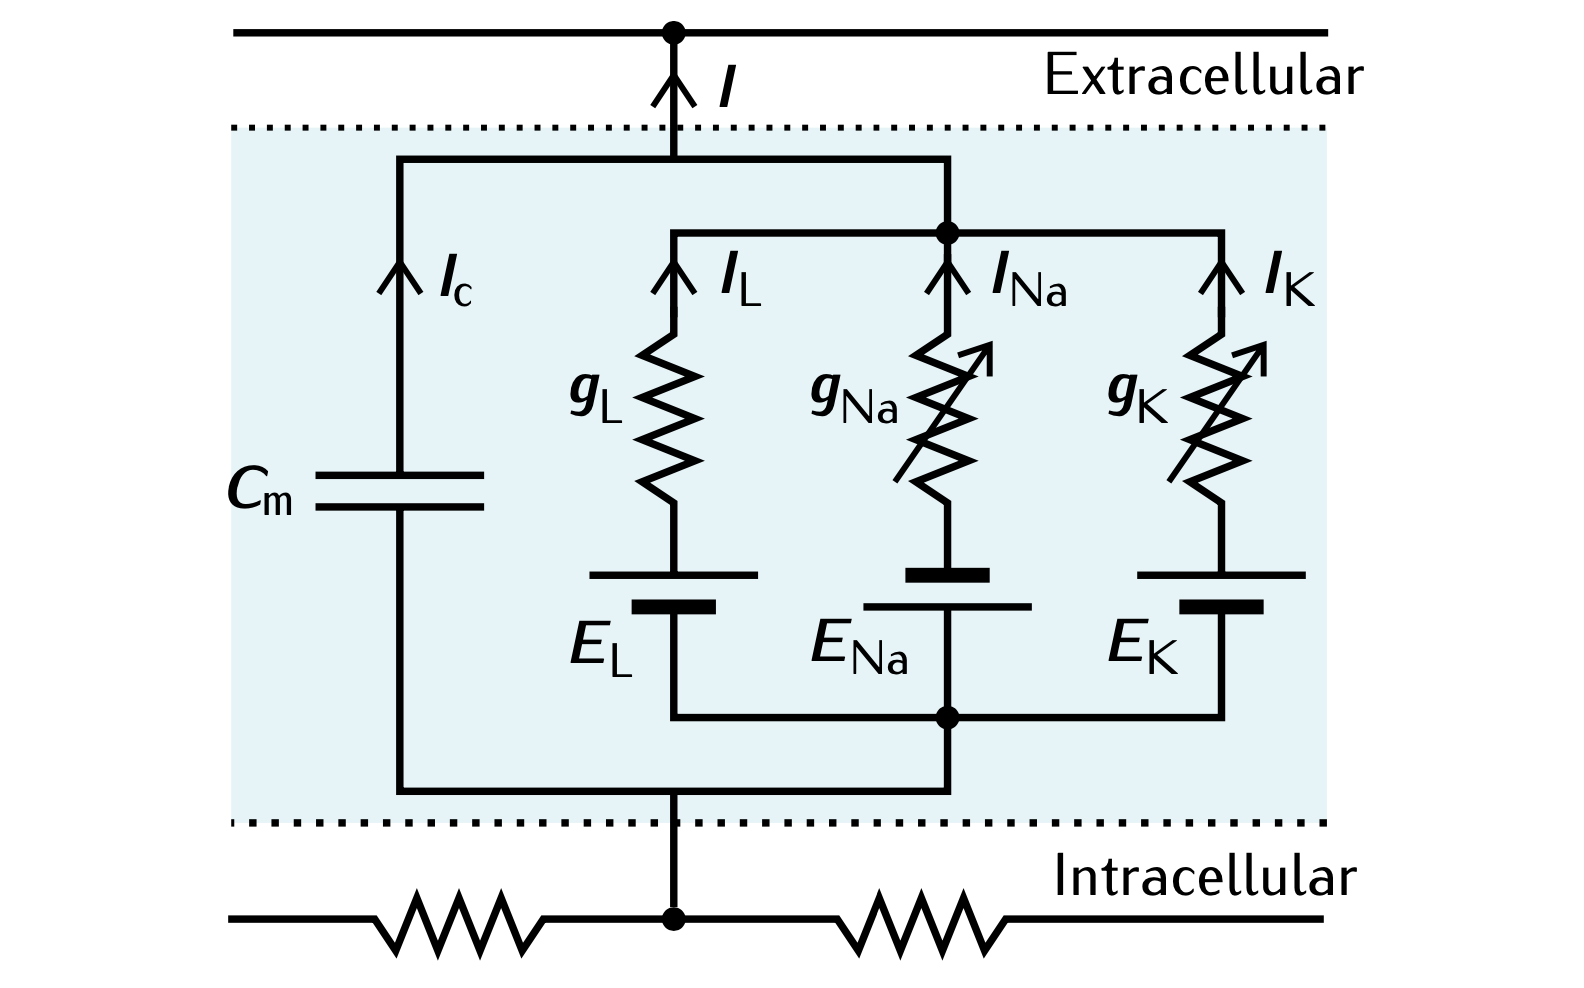
\includegraphics[scale=0.35]{hh_circuit}
    \caption{The HH equivalent circuit. 
    }
    \label{fig:hh_circuit}
    \source{\cite{Sterratt}.}
\end{figure}

Thus, the fundamental total current equation is:
\begin{equation}\label{eq:hh_total_current}
    \begin{aligned}
    I &= I_\mathrm{C} + I_\mathrm{K} + I_\mathrm{Na} + I_\mathrm{L} 
    \\
    &= C_m \frac{\dd{V}}{\dd{t}} + g_\mathrm{K} \qty(V - E_\mathrm{K}) + g_\mathrm{Na} \qty(V - E_\mathrm{Na}) + g_\mathrm{L} \qty(V - E_\mathrm{L})
    \end{aligned}
\end{equation}

In voltage-gated ion channels, the channel conductance $g_\mathrm{X}$ is a function of both voltage and time, $g_\mathrm{X} (V, t)$. We can write the time-dependent conductances like: 

\begin{equation*}
    g_\mathrm{X} (V, t) = \bar{g}_\mathrm{X} p_\mathrm{X} (V, t),
\end{equation*}

where $\bar{g}_\mathrm{X}$ is the total conductance when all channels of type $\mathrm{X}$ are fully open, i.e., the \textit{maximum conductance}, and $p_\mathrm{X} (V, t)$ is the fraction of channels of type $\mathrm{X}$ that are open, i.e., the \textit{channel density} (a number between 0 and 1). Hodgkin and Huxley suggested that the opening and closing of the voltage-gated ion channels were controlled by one or more \textit{gating particles}. Using a series of voltage clamp experiments, i.e., where the membrane potential is held at a level determined by the experimenter, and clever ionic substitutions, they were able to isolate the voltage-gated conductances of potassium and sodium. They obtained rate constants for the opening, closing and inactivation of the conductances by analyzing the voltage-dependence using first-order kinetics, and reduced these rate constants to a set of four ordinary differential equations:

\begin{subequations}\label{eq:hh_model}
    \begin{align}
    C_m \frac{\dd{V}}{\dd{t}} &= - \gbarK n^4 \qty(V - E_\mathrm{K}) - \gbarNa m^3h \qty(V - E_\mathrm{Na}) - \bar{g}_\mathrm{L} \qty(V - E_\mathrm{L}) + I
    \label{eq:hh_model_dVdt}
    \\
    \frac{\dd{n}}{\dd{t}} &= \alpha_n (V) (1-n) - \beta_n (V) n 
    \label{eq:hh_model_dndt}
    \\
    \frac{\dd{m}}{\dd{t}} &= \alpha_m (V) (1-m) - \beta_m (V) m
    \label{eq:hh_model_dmdt}
    \\
    \frac{\dd{h}}{\dd{t}} &= \alpha_h (V) (1-h) - \beta_h (V) h
    \label{eq:hh_model_dhdt}
    \end{align}
\end{subequations}

where the gating variables $n$, $m$ and $h$ are dimensionless quantities that are associated with potassium channel activation, sodium channel activation and sodium channel inactivation, respectively. The gating variables $n$ and $m$ range from $0$ (not activated) to $1$ (fully activated) and $h$ ranges from $0$ (fully inactivated) to $1$ (no inactivation). The voltage-dependent rate constants $\alpha_x (V)$ and $\beta_x(V)$, where $x \in \qty{n,m,h}$, represent the activation and inactivation rates, respectively, for gate $x$. \autoref{eq:hh_model} describes how the membrane potential $V$ across a membrane with capacitance $C_m$ responds to an input current $I$. Note that \autoref{eq:hh_model_dVdt} has been slightly reorganized from the formulation of the total current equation (\autoref{eq:hh_total_current}) to better reflect this. The potassium current, $I_\mathrm{K}$, is controlled by four identical gating particles, whereas the sodium current, $I_\mathrm{Na}$, is controlled by three identical and one distinct gating particle. The leak current, $I_\mathrm{L}$, is not voltage-dependent, and no gating particles are therefore associated with its conductance.

The forms of the $\alpha_x$ and $\beta_x$ functions were empirically proposed by the authors to fit the experimental recordings, yielding the following equations for the rate constants associated with the potassium activation gating variable;

\begin{subequations}
    \begin{align}
        \alpha_n (V) &= 0.01 \frac{V + 55}{1 - \exp \qty(-(V+55)/10)}
        \\
        \beta_n (V) &= 0.125 \exp \qty(-(V+55)/10)
    \end{align}
\end{subequations}

and for the sodium activation and inactivation gating variables: 

\begin{subequations}
    \begin{align}
        \alpha_m (V) &= 0.1 \frac{V + 40}{1 - \exp \qty(-(V+40)/10)}
        \\
        \beta_m (V) &= 4 \exp \qty(-(V+65)/18)
        \\
        \alpha_h (V) &= 0.07 \exp \qty(-(V+65)/20)
        \\
        \beta_h (V) &= \frac{1}{\exp \qty(-(V+35)/10) + 1}
    \end{align}
\end{subequations}


Here, we use a formulation of the model where the membrane voltage has been reversed in polarity from the original HH convention and shifted to reflect a resting potential of $-65 \mV$. An example of how to arrive at the alternative formulation is provided in \autoref{sec:Appendix B}. The original model parameter values are summarized in \autoref{tab:hh_model_parameters}.

\begin{table}[!htb]
  \caption{The original parametrization of the HH model.}
  %\footnotesize%
  \begin{center}
    \rowcolors{2}{gray!15}{white}
    \begin{tabular}{lll}
      \toprule
      \textbf{Parameter} & \textbf{Value} & \textbf{Description} \\
      \midrule
      $C_m$ & $1.0 \, \mathrm{\mu F \, cm}^{-2}$ & Membrane capacitance
      \\
      $\gbarK$ & $36.0 \gunit$ & Maximum potassium channel conductance 
      \\
      $\gbarNa$ & $120.0 \gunit$ & Maximum sodium channel conductance 
      \\
      $\bar{g}_\mathrm{L}$ & $0.3 \gunit$ & Maximum leakage channel conductance
      \\
      $E_\mathrm{K}$ & $-77.0 \mV$ & Potassium reversal potential
      \\
      $E_\mathrm{Na}$ & $50.0 \mV$ & Sodium reversal potential
      \\
      $E_\mathrm{L}$ & $-54.4 \mV$ & Leak reversal potential
      \\
      \bottomrule
    \end{tabular}
  \end{center}
  \label{tab:hh_model_parameters}
\end{table}

%================================================================ 
\subsection{Simulation of Action Potentials}
%================================================================ 

\autoref{fig:hh_states} shows the numerical solutions of a simulation of the HH model. As seen in the top panel, the shape of the simulated action potentials match the description of an action potential (see \cref{sec:ion_ch_and_ap}) well. Besides reproducing action potentials, the HH model offers insights into the mechanisms underlying them. The middle panel shows how the gating variables change during the temporal evolution of the action potentials. At stimulus onset (starting at $t=10 \ms$), the initial depolarization of the membrane potential is due to the input current. When the depolarization is above the threshold (at about $-55 \mV$), the sodium current activates, as reflected in the increase in $m$. As the sodium reversal potential is far higher than the resting membrane potential, the driving force of the sodium current pushes the membrane potential to sharply increase. The slower potassium conductance, reflected by the gating variable $n$, activates after the sharp rise in membrane potential and allows potassium ions to flow out of the neuron because of the low potassium reversal potential. In addition, the repolarization of the membrane potential is also assisted by the inactivating sodium gating variable, $h$, which shuts off the sodium current. This drives the membrane potential quickly back down towards its resting state, but undershoots somewhat, due to the slow de-inactivation of the sodium current, to hyperpolarize the neuron. The final recovery involves a rapid deactivation of the sodium current and a slower deactivation of the potassium current. Eventually all the state variables and the membrane potential return to their resting states. The HH model also explains the refractory period. Relative to the duration of an action potential, the gating variables recover to their resting states slowly. During this period, it is harder to generate an action potential. In the initial recovery phase, an increasing voltage will not increase the sodium conductance, and hence the membrane potential, considerably due to the ongoing inactivation of the sodium current and the prolonged activation of the potassium current. As the state variables advances in their recovery toward the resting states, an action potential can be initiated but will have a lower peak voltage. 

\begin{figure}[H]
    \centering
    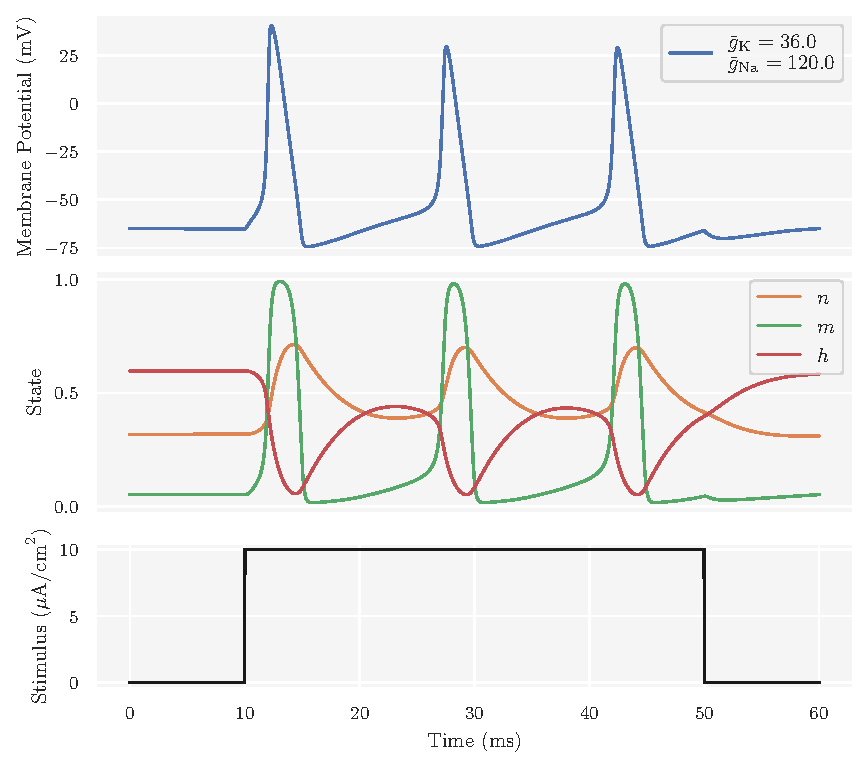
\includegraphics[scale=1.0]{hh_states}
    \caption{Simulated dynamics of $V$, $n$, $m$ and $h$ in the HH model during the firing of action potentials in the squid giant axon. The top panel shows the numerical solution of \autoref{eq:hh_model_dVdt} and the middle panel the numerical solutions of \Crefrange{eq:hh_model_dndt}{eq:hh_model_dhdt}. The system is simulated for $T = 60 \ms$ with time resolution $\Delta t=0.025 \ms$. The input stimulus received by the neuron (bottom panel) is a step current with amplitude $I = 10 \, \mathrm{\mu A/cm}^2$, and onset and offset at $10 \ms$ and $50 \ms$, respectively. The parametrization of the model is given by \autoref{tab:hh_model_parameters}. 
    }
    \label{fig:hh_states}
\end{figure}





%================================================================ 
%================================================================ 
%================================================================ 
%================================================================ 
%================================================================ 



%================================================================
\section{The Brunel Network Model}\label{sec:brunel_model}
%================================================================

Many neural networks of interest consist of thousands or millions of neurons, and, generally, it is infeasible to include all in the model. Neural network models are usually scaled down according to the ratio of different neuron populations in the network that the model tries to mimic. Furthermore, they often use simplified neuron models to reduce computational cost. Still, neural network models may exhibit a high diversity of spiking dynamics. In this section, we present one such model that is thoroughly analyzed in the literature; the Brunel network model \cite{Brunel2000}. Before we present the network model itself, we first discuss the central building block of the network: the leaky integrate-and-fire (LIF) neuron model. 


%================================================================
\subsection{Integrate-And-Fire Neurons}
%================================================================

While the ionic mechanisms behind APs are quite complicated, the conditions for AP generation are often quite straightforward: When the membrane potential reaches a specific threshold, a spike is generated and the membrane potential returns to the background state. Simulations of APs can be accelerated significantly by not explicitly modeling the responsible biophysical mechanisms. \textit{Integrate-and-fire} (IF) models are simplified neuron models with a spike generation and reset mechanism. In these models, whenever the membrane potential of a neuron reaches a threshold value $\theta$, a spike is generated and the membrane potential is reset to a value $V_\mathrm{reset}$ below the threshold potential, $V_\mathrm{reset} < \theta$. In the simplest IF model, all active membrane conductances are ignored and the entire membrane conductance is modeled as a single passive leakage conductance: 

\begin{equation*}
    I_\mathrm{L} = \bar{g}_\mathrm{L} \qty(V - E_m),
\end{equation*}

where $E_m$ is the resting membrane potential. Since the conductance is the reciprocal of the resistance, the above equation can be equivalently formulated as: 

\begin{equation*}
    I_\mathrm{L} = \frac{V - E_m}{R_m},
\end{equation*}

where $R_m$ is the membrane resistance. Furthermore, we assume that the model neuron behaves like an electric circuit consisting of a resistor and a capacitor in parallel, i.e., an RC circuit, driven by a current $I$. In addition, the circuit needs a switch, representing the reset mechanism, which is open until the membrane potential reaches $\theta$ and then closes to short-circuit the membrane resistance, bringing the membrane potential back to rest. The switch opens again after a refractory period $\tau_\mathrm{rp}$, allowing the membrane to charge. This neuron model is often called the \textit{leaky integrate-and-fire} (LIF) model. The circuit diagram and the RC circuit response to input stimulus is shown in \autoref{fig:lif_circuit}. When the membrane potential is below the threshold, its value is determined by the equation for an RC circuit: 

\begin{figure}[!htb]
    \centering
    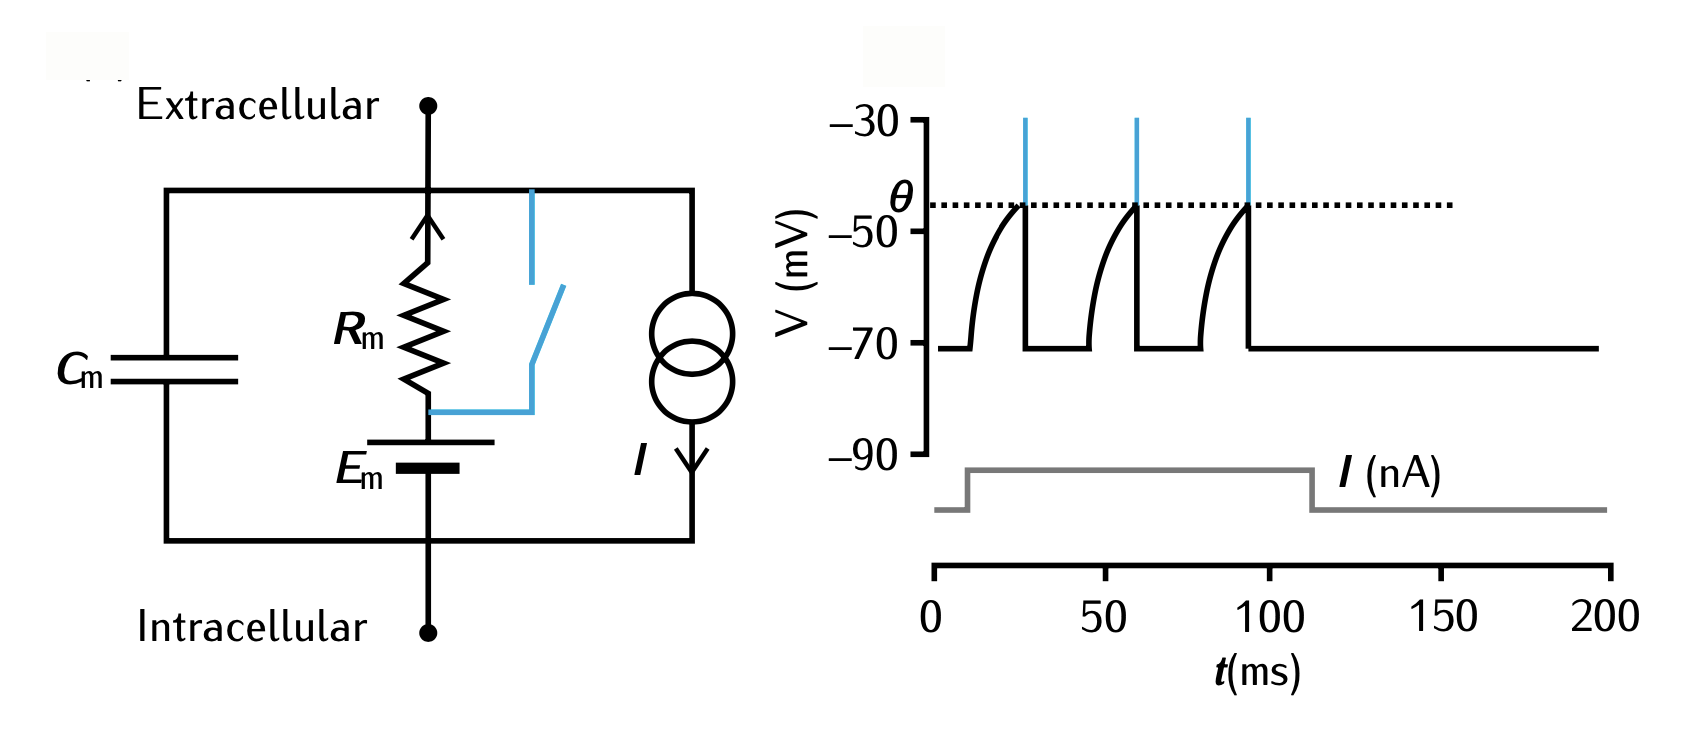
\includegraphics[scale=0.45]{lif_circuit}
    \caption{The LIF neuron model as an RC circuit diagram (left) with a switch (in blue on the diagram) and the response of the LIF neuron to input stimulus (right). When the switch is open, the membrane can charge. When the membrane potential reaches the threshold $\theta$ (indicated by the dashed line in the voltage trace), the neuron fires a spike (indicated by the vertical blue line in the voltage trace) and the switch closes. This short-circuits the membrane resistance, bringing the membrane potential back to its resting state. After a refractory period, the switch opens, allowing the membrane to charge again.
    }
    \label{fig:lif_circuit}
    \source{\cite{Sterratt}.}
\end{figure}

\begin{equation*}
    C_m \frac{\dd{V}}{\dd{t}} = - \frac{V-E_m}{R_m} + I.
\end{equation*}

The above equation is usually written in terms of the membrane time constant, $\tau_m = C_m R_m$: 

\begin{equation*}
    \tau_m \frac{\dd{V}}{\dd{t}} = - V + E_m + R_m + I.
\end{equation*}

Furthermore, the leak battery is often omitted from the circuit, with the only effect of making the resting membrane potential $0\mV$ instead of $E_m$: 

\begin{equation}\label{eq:lif_model}
    \tau_m \frac{\dd{V}}{\dd{t}} = - V + R_m + I.
\end{equation}

The simple LIF neuron model only captures the timing of each spike, but is fast to simulate compared to biophysically detailed neuron models. This makes it especially useful for simulating large networks, as these often contain thousands of neurons. 



%================================================================
\subsection{A Sparsely Connected Recurrent Network}\label{sec:recurrent_network}
%================================================================

The local cortical network consists of a population of excitatory neurons and a population of inhibitory neurons, with a ratio of about $80\%$ excitation and $20\%$ inhibition. The Brunel model characterizes the local cortical network as a network of $N$ identical LIF neurons, from which $N_E$ are excitatory and $N_I = N_E / 4$ inhibitory. Each neuron, be it excitatory or inhibitory, receives $C$ randomly connections from other neurons in the network, from which $C_E = \epsilon N_E$ are from the excitatory population and $C_I = \epsilon N_I$ from the inhibitory population. Here, $\epsilon$ denotes the fraction of incoming connections, and we consider a sparsely connected network with $\epsilon = C_E / N_E = C_I / N_I << 1$. In addition to the sparse recurrent inputs from within the local network, each neuron receives excitatory synaptic input from a population of $C_E$ randomly firing neurons outside the network with activation governed by identical, independent Poisson processes (PGs) with fixed-rate $\nu_\mathrm{ext}$. The randomly firing population mimics input from the rest of cortex. An illustration of the network is shown in \autoref{fig:brunel_diagram}.

\begin{figure}[!htb]
    \centering
    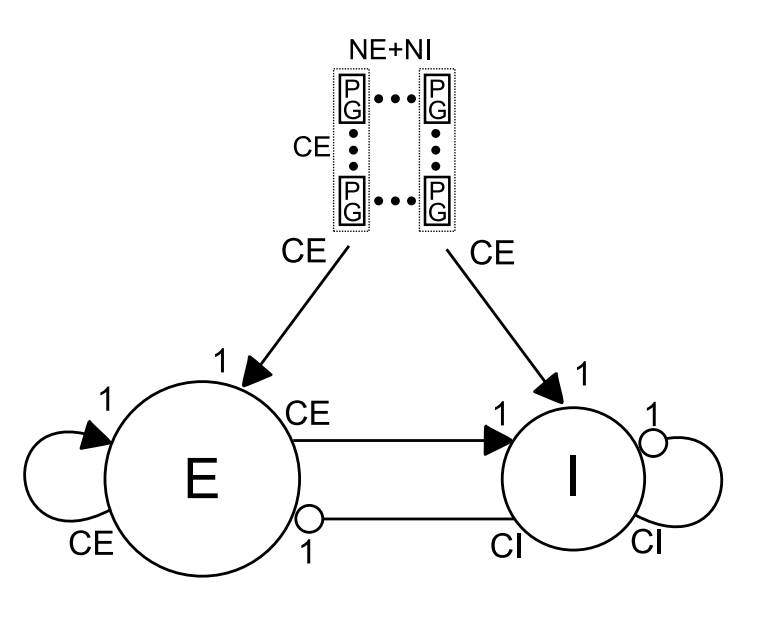
\includegraphics[scale=0.5]{brunel_diagram}
    \caption{Illustration of the Brunel network model. The network consists of two local populations, one with $N_E$ excitatory neurons (circle labeled E) and one with $N_I$ inhibitory neurons (circle labeled I), and one external population of identical, independent Poisson processes (PGs). The connections between network nodes are indicated by arrows, where triangular arrow-heads represent excitatory and round arrow-heads inhibitory connections. The numbers at the start and end of each arrow indicate the multiplicity of the connection.
    }
    \label{fig:brunel_diagram}
    \source{\cite{nest_by_example}.}
\end{figure}

The subthreshold dynamics of LIF neuron $i$ in the network ($i=1, ..., N$) evolves in time according to:

\begin{equation}
    \tau_m \frac{\dd{V_i (t)}}{\dd{t}} = - V_i(t) + R_m I_i(t),
\end{equation}

where $I_i$ are the synaptic inputs arriving at the soma. These synaptic inputs are the sum of spike contributions from both local and external synapses, and are modeled as $\delta$-current inputs, i.e., discontinuous voltage jumps: 

\begin{equation}
    R_m I_i (t) = \tau_m \sum_j J_{ij} \sum_k \delta \qty(t - t_j^k - D),
\end{equation}

where the first sum is over all the presynaptic neurons $j$ with postsynaptic potential amplitude (voltage jump) $J_{ij}$, while the second sum is over the spike times of those neurons. Here, $D$ is the synaptic delay, $\delta(x)$ the Dirac $\delta$ function, with $\delta(x)=0$ for $x \neq 0$ and $\int_{-\infty}^\infty \delta (x) \dd{x} = 1$, and $t_j^k$ represents the emission time of the $k$th spike of presynaptic neuron $j$. For simplicity, we assume the synaptic connection strengths are constant for each population. We let $J_{ij}=J>0$, and for excitatory neurons and external input $J_E = J$, while for inhibitory neurons $J_I = -g J_E$, where $g$ determines the relative strength of the inhibitory synapses compared to the excitatory synapses. The amount of input the local neurons receive from the external population is determined by the parameter $\eta = \nu_\mathrm{ext}/\nu_\mathrm{thr}$, where $\nu_\mathrm{thr} = \theta / \qty(J_E C_E \tau_m)$ is the minimum constant rate input needed for a neuron to reach threshold in absence of feedback. Thus, the external input rate is given by $\nu_\mathrm{ext} = \qty(\eta \theta) / \qty(J_E C_E \tau_m)$.  

When the membrane potential $V_i (t)$ of LIF neuron $i$ reaches the firing threshold $\theta$, the neuron fires a spike, the synapses onto all its postsynaptic neurons are activated after a time delay $D$ and the neuron's membrane potential is clamped to the reset potential $V_\mathrm{reset}$ for a refractory period $\tau_\mathrm{rp}$.


%================================================================
\subsection{States of Spiking Activity}
%================================================================

The Brunel network may be in several different states of spiking activity, largely dependent on the values of the synaptic weight parameters. In the context of a biological neural network, synaptic weight parameters refer to parameters that determines the influence the firing of one neuron has on another. With particular fixed values for $J$ and $D$ and varying values for $\eta$ and $g$, Brunel \cite{Brunel2000} characterized the spiking activity of the network by phase diagrams. An example of these is shown in \autoref{fig:brunel_phase}. The spiking activity can be in a state of synchronous regular (SR), asynchronous irregular (AI) or synchronous irregular (SI), with either fast or slow oscillations, activity. It can be seen from the phase diagram that $g=4$ corresponds to balance between excitation and inhibition, while $\eta=1$ corresponds to external input, in the absence of recurrent input from the network, just sufficient to reach the firing threshold. Stability of the AI state breaks down at the dashed or solid lines and can lead to SR or SI (either fast or slow) activity.

\begin{figure}[!htb]
    \centering
    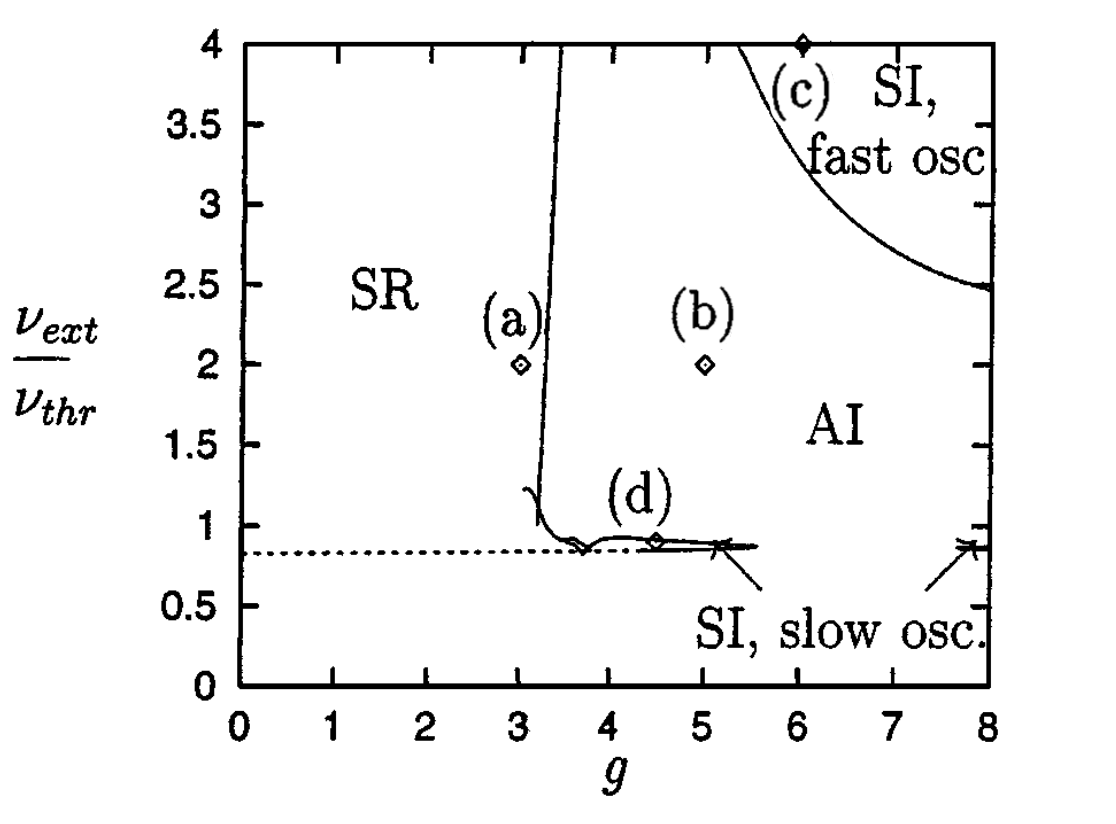
\includegraphics[scale=0.45]{brunel_phase}
    \caption{Phase diagram of different network states which arise depending on the parameters $\eta = \nu_\mathrm{ext}/\nu_\mathrm{thr}$ and $g$. In the present example, a fixed synaptic delay $D=1.5\ms$ and voltage jump (amplitude of excitatory synaptic input currents)  $J_E = 0.1 \mV$ is used. The simulation is of a network consisting of $N_\mathrm{E}=10,000$ excitatory and $N_\mathrm{I} = 2,500$ inhibitory neurons with connection probability $\epsilon = 0.1$, which corresponds to a network where each neuron has $C_\mathrm{E}=1,000$ and $C_\mathrm{I}=250$ randomly selected connections to excitatory and inhibitory neurons, respectively. The phase diagram shows four states of spiking activity: synchronous regular (SR), asynchronous irregular (AI) and of synchronous irregular (SI), fast and slow. The four points (shown by diamonds) indicate the example activities shown in \autoref{fig:brunel_states}.
    }
    \label{fig:brunel_phase}
    \source{\cite{Brunel2000}.}
\end{figure}

\autoref{fig:brunel_states} illustrates an example of each of the states of the Brunel network. For each state, the figure shows the firing times (rasters) of 20 randomly chosen excitatory neurons, the temporal evolution of the activity in the network (time resolved firing rate computed in bins of 10 ms) together with the mean firing rate (horizontal axis line), and the pairwise Pearson's correlation coefficient matrix (described in the next chapter) of the recorded neurons. The particular values for $\eta$ and $g$ are stated in the subplot titles and correspond to the points (diamonds) in \autoref{fig:brunel_phase}. In the SR state, the network is almost fully synchronized and the neurons fire at high rates. It is characterized by fast periodic oscillations of the spiking activity. In the AI state, neurons fire mostly independently at low rates. It is characterized by that neurons in the population fire at different times (\textit{asynchronous firing}) and at irregular intervals. In the SI states, the spiking activity of the network is characterized by either fast or slow synchrony, but individual neurons fire irregularly. It can be traced back to an instability of the AI firing regime towards oscillatory activity. The pairwise Pearson's correlation coefficient measures the correlation between spike trains of two neurons in the network, and can be used to examine how synchronous the spiking of a network is. We see that in the SR state, the correlation coefficients are much higher than in the AI state. The SI state with fast oscillations, however, is only scarcely more synchronous than the AI state. The SI state with slow oscillations, on the other hand, has increased synchrony compared to the AI state. 

\begin{figure}[H]
    \centering
    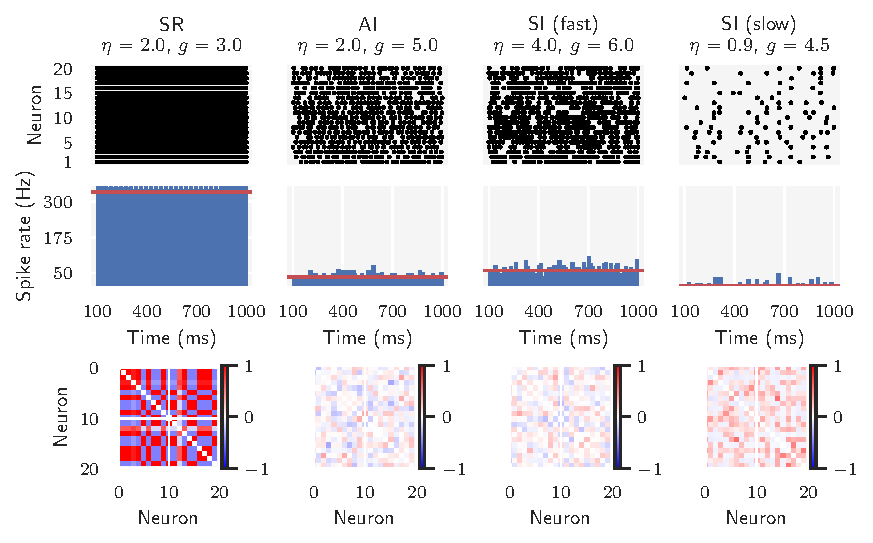
\includegraphics[scale=1.0]{brunel_states}
    \caption{Simulation of the network specified by \autoref{tab:bnet_model_parameters}, with the values of $\eta$ and $g$ stated in each subplot's title along with the network state. The network is simulated for $T_\mathrm{sim} = 1,000$ ms, and we record the output from $N_\mathrm{rec} = 20$ excitatory neurons. To avoid transient effects, we start recording after $T_\mathrm{transient} = 100$ ms. The top row shows the firing times (raster) of the recorded neurons. Each point in the raster corresponds to the firing of a neuron. The second row shows the network activity as a time resolved firing rate computed in bins of $10 \ms$. The mean firing rate is indicated by the horizontal (red) axis line. The third row shows the pairwise Pearson's correlation coefficient matrix of the recorded neurons.
    }
    \label{fig:brunel_states}
\end{figure}


\autoref{tab:bnet_model_parameters} summarizes the parametrization of the Brunel model used in the above simulations.

\begin{table}[!htb]
  \caption{The parametrization of the Brunel model. Specific values are not provided for the parameters derived from the varying $\eta$ and $g$.}
  %\footnotesize%
  \begin{center}
    \rowcolors{2}{gray!15}{white}
    \begin{tabular}{lll}
      \toprule
      \textbf{Parameter} & \textbf{Value} & \textbf{Description} \\
      \midrule
      $N$ & $12,500$ & Total number of neurons
      \\
      $N_E$ & $10,000$ & Number of excitatory neurons
      \\
      $N_I$ & $2,500$ & Number of inhibitory neurons
      \\
      $\epsilon$ & $0.1$ & Connection probability
      \\
      $C_E$ & $1,000$ & Excitatory synapses per neuron
      \\
      $C_I$ & $200$ & Inhibitory synapses per neuron
      \\
      $E_m$ &  $0 \mV$ & Resting membrane potential 
      \\
      $C_m$ &  $1 \, \mathrm{pF}$ & Membrane capacitance
      \\
      $\tau_m$ &  $20 \ms$ & Membrane time constant
      \\
      $\theta$ &  $20 \mV$ & Firing threshold
      \\
      $V_\mathrm{reset}$ &  $10 \mV$ & Reset membrane potential
      \\
      $\tau_\mathrm{rp}$ &  $2 \ms$ & Refractory period
      \\
      $D$ &  $1.5 \ms$ & Synaptic delay
      \\
      $J_E$ &  $0.1 \mV$ & Excitatory synapse strength
      \\
      $J_I$ &  $-g J_E$ & Inhibitory synapse strength
      \\
      $\nu_\mathrm{ext}$ &  $\qty(\eta \theta)/\qty(J_E C_E \tau_m)$ & External firing rate
      \\
      \bottomrule
    \end{tabular}
  \end{center}
  \label{tab:bnet_model_parameters}
\end{table}
